\section{Random Variation in Genetic Inheritance}
\label{sec:genetics}
Genetic variants are not randomly assigned, which means that simple correlations between the Ed PGI and outcomes cannot be interpreted as causal relationships.
Genes are inherited from parents, where children receive 23 chromosomes from each parent at conception --- half the genes from their mother, half from father.
This inheritance pattern creates systematic associations between an individual's genetics and their family environment, as children who inherit certain genetic variants also inherit the familial circumstances from parents carrying those variants.
However, this inheritance pattern also involves independent random variation, which I use to instrument for changes in the Ed PGI and thus estimate causal effects.

\subsection{Mendelian Independent Inheritance}
I use variation away from parental values to estimate causal effects of having a higher versus lower Ed PGI.
This approach leverages the fundamental randomness in genetic inheritance, first described by Mendel's laws \citep{mendel1865versuche}.

\begin{figure}[h!]
    \centering
    \singlespacing
    \caption{Mendelian Independent Inheritance of One Genetic Variant.}
    \label{fig:mendelian-indep}
    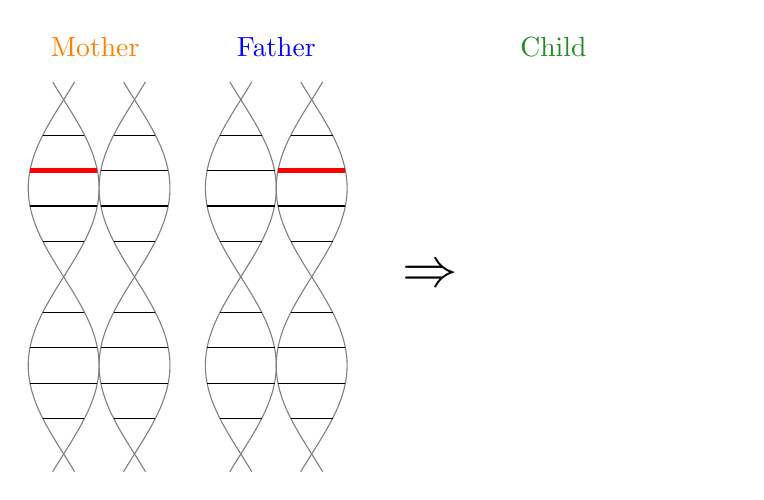
\begin{tikzpicture}
    % Draw the mother + father 
        \begin{scope}[scale=0.45, domain=-0.5:10.5, samples=110, rotate=90]
        %% Father
        \node[text width=1.0cm, color=blue] at (11.5, 0) {Father};
        %% Mother
        \node[text width=1.0cm, color=orange] at (11.5, 0 + 5.25) {Mother};
        % Draw the phosphate backbone, for each chromosome.
        \draw[gray] plot (\x,{sin(\x*36) + 1});
        \draw[gray] plot (\x,{-sin(\x*36) + 1});
        \draw[gray] plot (\x,{sin(\x*36) - 1});
        \draw[gray] plot (\x,{-sin(\x*36) - 1});
        % Draw the base pairs bonds
        \foreach \x in {0, 1, ..., 10}{
            \draw (\x, {-sin(\x*36) + 1}) -- (\x, {sin(\x*36) + 1});
            \draw (\x, {-sin(\x*36) - 1}) -- (\x, {sin(\x*36) - 1});
        }
        % Draw the phosphate backbone for mother
        \draw[gray] plot (\x, {sin(\x*36) + 4});
        \draw[gray] plot (\x, {-sin(\x*36) + 4});
        \draw[gray] plot (\x, {sin(\x*36) + 6});
        \draw[gray] plot (\x, {-sin(\x*36) + 6});
        % Draw the base pairs bonds
        \foreach \x in {0, 1, ..., 10}{
            \draw (\x, {-sin(\x*36) + 4}) -- (\x, {sin(\x*36) + 4});
            \draw (\x, {-sin(\x*36) + 6}) -- (\x, {sin(\x*36) + 6});
        }
        % Draw the one copy on each parent, at j = 8.
        \foreach \x in {8}{
            \draw[red, ultra thick] (\x, {-sin(\x*36) - 1}) -- (\x, {sin(\x*36) - 1});
            \draw[red, ultra thick] (\x, {-sin(\x*36) + 6}) -- (\x, {sin(\x*36) + 6});
        }
    %% Bridge to the child's genome
    \node[text width=2cm, scale=2] at (5, -8) {$\Rightarrow$};
    \node[text width=1.0cm, scale=1, color=ForestGreen] at (11.5, -8) {Child};
    \end{scope}
\end{tikzpicture}

    \justify
    \footnotesize
    \textbf{Note}:
    This figure illustrates the process of Mendelian Independent Inheritance of genetic variants, for parents with each one copy of a variant (red) and the resulting possibilities for their child's inherited variants.
\end{figure}

Each parent has 0, 1, or 2 copies of each genetic variant --- corresponding to presence on each of their chromosomes.
When a father and mother's sex cells are formed, exactly one of the two copies is sorted into each reproductive cell, and is then inherited by their resulting child.
A parent with one copy therefore passes it on half the time, whereas a parent with 0 or 2 copies transmits their genetic variant with certainty.
At conception, the child receives one draw from the mother and one from the father, so the child's copy-count is simply the sum of two independent draws.

Write $x_{i,j}^\text{\textcolor{ForestGreen}{Child}}$ for the number of copies of variant $j$ that individual $i$ has (0, 1, or 2), and 
$x_{m(i),j}^\text{\textcolor{orange}{Mother}}, x_{f(i),j}^\text{\textcolor{blue}{Father}}$ for their respective parents $m(i), f(i)$.
If the mother has two copies of variant $j$ then they bequeath one copy to their child with certainty; if the father has one, then they bequeath one copy with probability $\frac 12$; if no copies, then they bequeath none with certainty.
\[ \Egiven{x_{i,j}^\text{\textcolor{ForestGreen}{Child}}}{
    x_{m(i),j}^\text{\textcolor{orange}{Mother}},
        x_{f(i),j}^\text{\textcolor{blue}{Father}}}
    = \Egiven{x_{i,j}^\text{\textcolor{ForestGreen}{Child}}}{
        x_{f(i),j}^\text{\textcolor{blue}{Father}}}
    + \begin{cases}
        0, &\text{ if } x_{m(i),j}^\text{\textcolor{orange}{Mother}} = 0 \\
        \frac 12, &\text{ if } x_{m(i),j}^\text{\textcolor{orange}{Mother}} = 1 \\
        1, &\text{ if } x_{m(i),j}^\text{\textcolor{orange}{Mother}} = 2.
    \end{cases} \]
The child then receives their other copy from their father, by the same process, giving the following representation in expectation,
\[ \Egiven{x_{i,j}^\text{\textcolor{ForestGreen}{Child}}}{
    x_{m(i),j}^\text{\textcolor{orange}{Mother}}, x_{f(i),j}^\text{\textcolor{blue}{Father}}}
    = \frac 12 \Big( x_{m(i),j}^\text{\textcolor{orange}{Mother}}
        + x_{f(i),j}^\text{\textcolor{blue}{Father}} \Big). \]

After conception, the child has inherited genetic variants from both parents --- the discrete realisation, and not the expected value.
This result came about purely from random chance, conditional on at least one of parent having exactly one copy of the SNP, $x_{m(i),j}^\text{\textcolor{orange}{Mother}} = 1$ and/or $x_{f(i),j}^\text{\textcolor{blue}{Father}} = 1$.\footnote{
    Note both parents having 0 or 2 copies leaves $x_{i',j'}^\text{\textcolor{red}{Random}} = 0$, so that individual $i'$ inherited no random variation in variant $j'$.
}
\[ x_{i,j}^\text{\textcolor{red}{Random}}
    \coloneqq x_{i,j}^\text{\textcolor{ForestGreen}{Child}}
    - \Egiven{x_{i,j}^\text{\textcolor{ForestGreen}{Child}}}{
        x_{m(i),j}^\text{\textcolor{orange}{Mother}},
            x_{f(i),j}^\text{\textcolor{blue}{Father}}}
    \;\; \longrightarrow \;\; \text{Independently assigned.} \]
$x_{i,j}^\text{\textcolor{red}{Random}}$ is the random variation in presence of SNP at position $j$.
From the possible values of the parents' variants, $x_{i,j}^\text{\textcolor{red}{Random}}$ equals zero if both parents have 0 or 2 copies, equals $\frac 12$ if the child actually inherited 1 copy when both parents had one copy each ($- \frac 12$ if they did not inherit), and 1 if they inherited 2 copies and the parents had one each ($-1$ if they inherited 0).

\subsubsection{Mendelian Independent Inheritance in the Ed PGI}
Moving from a single variant to the PGI simply means summing across the same random-segregation for all the variants.
The Ed PGI is constructed by summing the 0, 1, or 2 copy indicators across the $J \approx 8,000$ different SNPs, each multiplied by the externally estimated weights $w_{i,j}$ that capture how strongly each SNP predicts education years.
Because every variant copy enters the child's genome through an independent random draw (conditional on parental values), the child's Ed PGI is the weighted sum of thousands of such draws.

This means the Ed PGI can be decomposed into the component that was inherited as a result of a random draws from parent(s) who had 1 copy of the variant, and the certainty component from draws where parent(s) had 0 or 2 copies.
\[ Z_i^\text{\textcolor{ForestGreen}{Child}}
    = Z_i^\text{\textcolor{red}{Random}}
        + \Egiven{Z_i^\text{\textcolor{ForestGreen}{Child}}}{
            Z_{m(i)}^\text{\textcolor{orange}{Mother}},
                Z_{f(i)}^\text{\textcolor{blue}{Father}}}, \]
where $Z_i^\text{\textcolor{red}{Random}} = \sum_{j = 1}^J w_j x_{i,j}^\text{\textcolor{red}{Random}}$ is the random component of the Ed PGI for individual $i$, and similarly for their parents' Ed PGI values, $Z_{m(i)}^\text{\textcolor{orange}{Mother}}$ and $Z_{f(i)}^\text{\textcolor{blue}{Father}}$.
$Z_i^\text{\textcolor{red}{Random}}$ is the random component because it was the result of Mendelian independent inheritance, and its only determining factor was having at least one parent with exactly one copy for relevant genetic variants --- and nothing else.

\begin{figure}[h!]
    \centering
    \singlespacing
    \caption{Correlation for Ed PGI, or Random Component, and Demographic Variables.}
    \label{fig:demographic-correlates}
    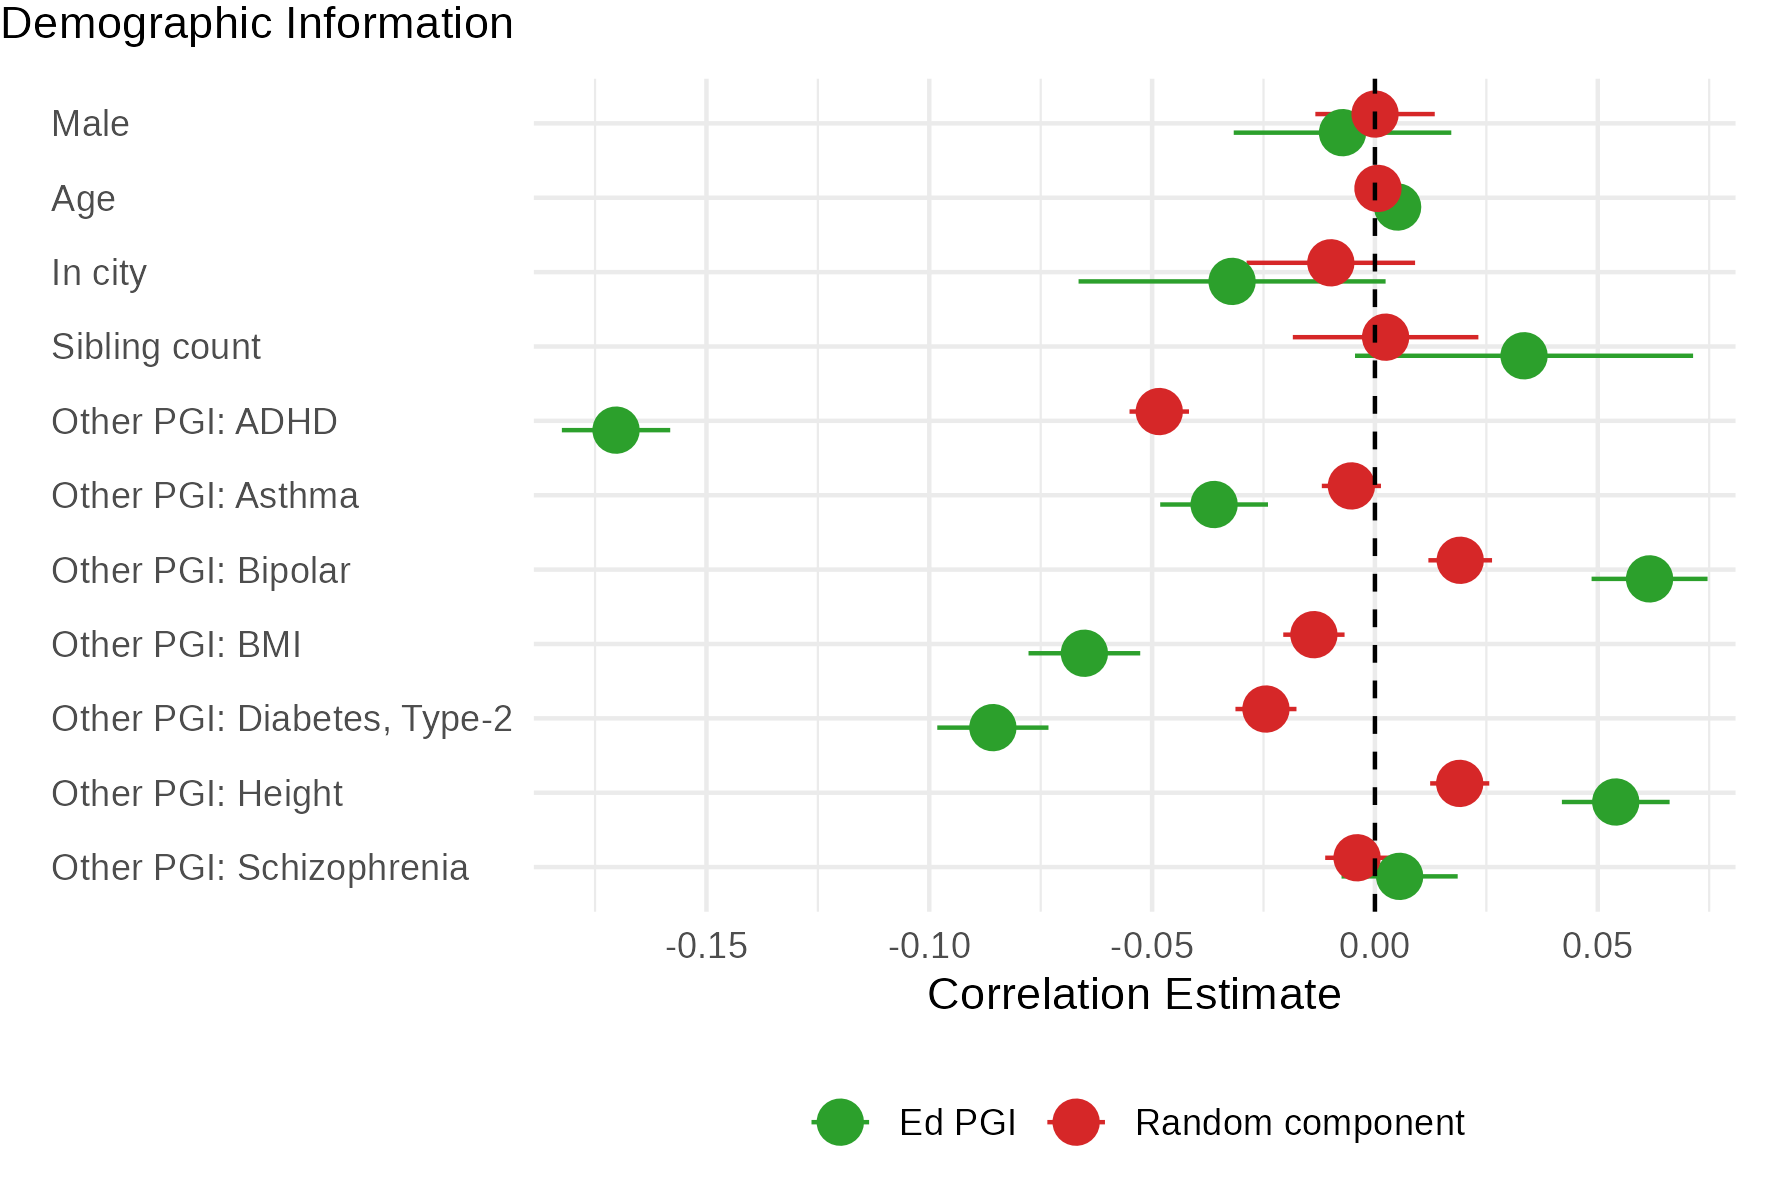
\includegraphics[width=0.85\textwidth]{sections/figures/demographic-correlates.png}
    \justify
    \footnotesize
    \textbf{Note}:
    Multivariate regression estimates for the linear model $Z_i = \beta\,' \, \vec X_i + \eta_i$, for each $Z_i^\text{\textcolor{ForestGreen}{Child}}$ and $Z_i^\text{\textcolor{red}{Random}}$, where $\vec X_i$ is the vector demographic variables described by the labels on the $y$-axis.
\end{figure}

\textbf{Describe the random component.
What is its distribution.
It is not correlated with other demographic variables, and less so with the other PGIs.}
\autoref{fig:demographic-correlates} shows what the Ed PGI, and the calculated random component is correlated with.

\subsubsection{Using Imputed Parental Ed PGI Values}
The random component is a function of parental PGI values, which are not directly observed in the UKB data.
I impute the mean of the parents value, $\frac 12 \big( Z_{m(i),j}^\text{\textcolor{orange}{Mother}} + Z_{f(i),j}^\text{\textcolor{blue}{Father}} \big)$, using the genetic data from individuals who have siblings in the UKB.
This is the method proposed by \cite{young2022mendelian}, who showed that the genotypes of a pair of siblings contain almost all the information needed.
For any given SNP the two children collectively reveal between two and four of the four parental variants, depending on how many variants the siblings share identically-by-descent (IBD).
Averaging over the three possible IBD states, the analyst observed 3 out of 4 variants in expectation; the final unobserved variant is imputed with its population frequency.
Taking weighted sums across the thousands of variants therefore yields imputed parental PGIs that are extremely highly correlated with the true parental values --- see \autoref{sec:pgi-impute}.

Substituting these imputed values in place of the missing parental values does not bias the downstream regression; \cite{young2022mendelian} the resulting estimators of the effects remain unbiased and consistent, and that the usual robust variance formula is valid.
The chief cost is a modest loss of precision: depending on genetic data availability, and the proportion of siblings' genetic variants that end up being identical-by-descent, the effective sample size is one-half to one-sixth of what it would be if both parents were actually observed.
Even so, this represents a substantial gain over the classical sibling-difference design.

The random genetic variation leveraged in this analysis fundamentally arises from siblings who inherit different sets of variants from their parents.
An individual and their sibling may inherit Ed PGI values far apart, from randomly one inheriting more copies of relevant variants from their than their sibling.
The resulting variation provides a natural experiment, offering a source of quasi-experimental variation.
In contrast, sibling pairs whose inherited Ed PGI values close to each other (or equal) produce minimal informative variation.
Thus, the effective random variation in this framework predominantly stems from sibling pairs whose genetic inheritance diverges notably.

Consequently, the derived random genetic component is inherently a noisy measure of true Mendelian random variation.
Its precision depends on how genetically distinct each sibling pair is: sibling pairs who differ widely provide clearer signals, while genetically similar pairs introduce greater measurement noise.
For estimation, an Ordinary Least Squares (OLS) regression estimate will implicitly weight observations by variance \citep{angrist1998estimating}, meaning sibling pairs with larger genetic differences carry greater influence on estimated effects.
The resulting estimates disproportionately reflect families where sibling genetic inheritance diverged substantially, potentially affecting generalisability if sibling genetic divergence correlates systematically with family characteristics.

\subsection{Measurement Error in the Ed PGI}
An important econometric consideration is that the Ed PGI weights, $w_{j'}$, are themselves statistical estimates rather than true population parameters.
Although the \cite{okbay2022polygenic} weights are estimates from an exceptionally large sample of over 3 million individuals, they remain subject to finite sample sampling variation and estimation error.
This measurement error in the weights propagates through to the constructed Ed PGI, resulting in classical attenuation bias when examining correlations between the PGI and outcomes of interest.

To address this measurement error problem, I follow Muslimova (2024) and construct a second Ed PGI using alternative weights, also provided by Okbay et al.
(2022), that were estimated exclusively from the UK Biobank non-sibling subsample.
Crucially, because these two sets of weights were estimated from independent samples, their measurement errors are uncorrelated.
This allows me to implement an Obviously Related Instrumental Variables (ORIV) approach, where each PGI serves as an instrument for the other, effectively trading off some statistical precision for reduced attenuation bias.
The ORIV estimator provides consistent estimates of the relationship between the true (error-free) Ed PGI and outcomes, correcting for the downward bias that would otherwise affect my results.
Appendix \ref{appendix:oriv} provides a detailed exposition of this econometric approach and its implementation in the context of PGIs.

\subsection{First-Stage Effects}

Draw the estimating first-stage equation,
\[ Z_i^\text{\textcolor{ForestGreen}{Child}}
    = \gamma + \theta Z_i^\text{\textcolor{red}{Random}}
        + \zeta Z_i^\text{Imputed}
            + \eta_i \]


Show first-stage estimates of random component on child PGI, show it using the random component of one Ed PGI onto the other.
First-column 1 on 2, second 2 on 1, third stacked obviously related.
This is then showing results which are not mechanical; in doing so I can also replace the empirical expectation with the raw mean imputed value (if it improves the F stats).

\begin{table}[h!]
    \singlespacing
    \centering
    \small
    \caption{First-stage Genetic Estimates,
        $Z_i^\text{\textcolor{red}{Random}} \to Z_i^\text{\textcolor{ForestGreen}{Child}}$ Independently and with ORIV.}
    \begin{tabular}{l c c c c c c}
        \\[-1.8ex]\hline \hline \\[-1.8ex] 
        & \multicolumn{6}{c}{Outcome:} \\
        & \multicolumn{3}{c}{Primary Ed PGI}
            & \multicolumn{3}{c}{Secondary Ed PGI} \\
        \cmidrule(lr){2-4} \cmidrule(lr){5-7}
        & (1) & (2) & (3) & (4) & (5) & (6) \\
        \midrule
        %\\[-1.8ex]\hline \\[-1.8ex]
        % latex table generated in R 4.5.1 by xtable 1.8-4 package
% Fri Jul 25 15:36:39 2025
 Primary Ed PGI, $Z_i^\text{\textcolor{red}{Random}}$ & 1 &   &   & 0.204 &   &   \\ 
    & (0.001) &   &   & (0.012) &   &   \\ 
  Secondary Ed PGI, $Z_i^\text{\textcolor{red}{Random}}$ &   & 0.158 &   &   & 1 &   \\ 
    &   & (0.011) &   &   & (0.001) &   \\ 
  Combined, ORIV &   &   & 1.336 &   &   & 1.495 \\ 
    &   &   & (0.043) &   &   & (0.048) \\ 
  \\[-1.8ex]\hline \\[-1.8ex] $F$-statistics &   & 207 & 971 & 305 &   & 957 \\ 
  $R^2$ & 0.998 & 0.091 &   & 0.051 & 0.994 &   \\ 
  Observations & 24755 & 24755 & 24755 & 24755 & 24755 & 24755 \\ 
  
        \\[-1.8ex]\hline \\[-1.8ex]
    \end{tabular}
    \vspace{-0.25cm}
    \label{tab:genetic-firststage}
    \justify
    \footnotesize
    \textbf{Note:}
    This table ...
\end{table}
